\documentclass{article}
\usepackage{csquotes}
\usepackage{hyperref}
\hypersetup{colorlinks=true,urlcolor=blue}
\usepackage{graphicx}
\graphicspath{ {images/} }
\usepackage[rightcaption]{sidecap}

\title{Chess Variants}
\author{Matthew Gallant}
\date{September 27, 2015}

\begin{document}
\maketitle

\section{Introduction}
These two variants of chess were created for the exercise ``Fog of Strategy'' in Chapter 8 of \textit{Challenges for Game Designers} by Brenda Brathwaite \& Ian Schreiber. The challenge given was:

\begin{displayquote}
For this challenge, choose an entirely skill-based, non-digital game with no elements of chance at all, such as \textit{Connect Four}, \textit{Chess}, or \textit{Go}. To adapt the game for less competitive players, you're going to add some chance. Specifically, add ``fog of war'': your opponent's pieces are hidden from you (and vice versa) except under certain conditions.
\end{displayquote}

\noindent\hfil\rule{0.5\textwidth}{.4pt}\hfil

\section{Luft Chess}

\begin{SCfigure}[0.8][h]
\caption{Example of luft, \textit{Wikipedia}.}
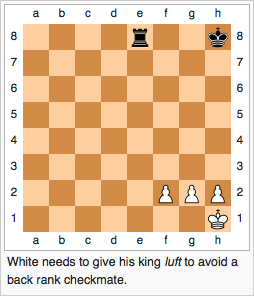
\includegraphics[width=0.35\textwidth]{luft}
\end{SCfigure}

\textit{Luft} (German for air, space or breath) is a chess term which denotes ``a space left by a pawn move into which a castled king may move''. In other words, it refers to intentionally leaving spaces open for the king to move into in the event of a back row check.

In this variant of chess, the king himself is made of air, and is thus invisible to the opposing player.

\subsection{Materials}
A standard chess set, two pieces of paper and two pens.

\subsection{Rules}
\textit{Luft Chess} is played with standard chess rules, with the following changes:

\begin{itemize}
\item The pieces are set up in the standard positions, except with blank spaces left for each player's invisible king. The king follows all the standard rules despite not being visible on the board (except as indicated below).
\item Players must tell their opponent when they move their king, but do not indicate where the king has moved. Each player secretly tracks the movement of their king on a separate piece of paper (for verification after the game, if necessary.)
\item Players may move their pieces through their own king, but may not place another piece at the same position.
\item If the opponent's move places your king in check or checkmate, you must tell them. However, you do not need to indicate the position of your king, nor which pieces are threatening it. If the opposing player moves a piece to the same position as your king, then the king is considered captured.
\item A king may not capture an opposing king, and a king is never considered threatened by an opposing king. Both players' kings may knowingly or unknowingly occupy the same position on the board.
\end{itemize}

\noindent\hfil\rule{0.5\textwidth}{.4pt}\hfil

\section{Reverse Schr\"{o}dinger's Chess}
When I began mulling over the ``Fog of Strategy'' challenge, my first idea was to create a variant of chess where players would secretly deploy their back line pieces at the beginning of the game, then gradually reveal those pieces as the game played out. Unfortunately, I discovered that this variant of chess already exists (\textit{\href{http://elvis.rowan.edu/~kilroy/other/?chess}{Schr\"{o}dinger's Chess}} by Darren Provine).

However, this led me to consider a modification of this variant. What if you secretly deployed your opponent's back row pieces, then revealed your own unknown pieces as the game played out?

\newpage

\subsection{Materials}
In addition to a standard chess set, players will need 7 black tokens and 7 white tokens. These tokens should indicate one of the seven available pieces on one side (2 knights, 2 bishops, 2 rooks, 1 queen) and be blank on the other. These pieces will be flipped over or substituted for the real pieces as the game progresses.

\begin{center}
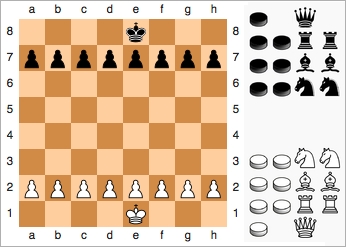
\includegraphics[width=0.5\linewidth]{reverse}
\end{center}

\subsection{Rules}
\textit{Reverse Schr\"{o}dinger's Chess} is played with standard chess rules, with the following changes:

\begin{itemize}
\item Rooks, bishops, knights and queens begin the game concealed. The six concealed pieces go in the usual locations, but are secretly rearranged by the \textbf{opposing} player at the start of the game.
\item Neither player may look at a concealed piece after the initial setup, until that piece is revealed.
\item When a player captures an opponent's piece, they must choose one of their own concealed pieces on the board and reveal it, if possible. Once revealed, a piece moves according to the traditional rules.
\end{itemize}

\noindent
It also inherits the following rules from standard \textit{Schr\"{o}dinger's Chess}:

\begin{itemize}
\item While concealed, pieces can move and capture one or two squares in any direction.
\item If a piece is captured while still concealed, it remains concealed until the game is over.
\item A concealed piece is considered ``concealed'', even if the other five concealed pieces have been revealed and there is no longer any doubt about what it is.
\item To castle, a rook must be uncovered and must be in either A or H.
\end{itemize}

\end{document}